
\section{User Training} \label{sec:BG:userTraining}

As user training in relation to prosthetic control is the main focus of this project an understanding of this concept in relation to receiving a prosthetic device is of great importance. Therefore the following section will cover an introduction to the concept of user training and its importance when preparing a subject to receive a prosthetic device. In addition, some of the prior techniques of conducting user training will be presented, facilitating the possibility of assembling a user training protocol based on the most recent and cutting edge results. \\
%user training and implementation
When fitting an amputee with a prosthesis, the way the prosthesis is controlled is important. A lot of work lies both before and after fitting a person with a prosthesis. When developing and manufacturing a prosthesis two concepts emerge, one being system training and the other being user training. System training is training the control system to be able to recognize and differ movements based on the EMG signal being fed to the system. \cite{Fougner2012} User training on the other hand focuses on training the user in performing distinguishable movements which can be recognized by the control system. Here different types of feedback can be used to inform the user on how well the user performs a movement or how the system recognizes the users performed movements. \cite{Powell2014,Simon2013} \\
%Copied from introduction 
Only few studies have earlier explored the optimal way of giving visual feedback in user training \cite{Jiang2012}. In a 2014 study Powell et al. \cite{Powell2014} provided the user with real-time visual feedback of a virtual prosthesis. This type of feedback is similar to the visual feedback a prosthesis user would receive using a normal prosthesis, although without the sensory feedback of the weight of the prosthesis. An illustration of the setup used in \cite{Powell2014} can be seen in \figref{fig:PowellUserTraining}.

\begin{figure}[H]                 
	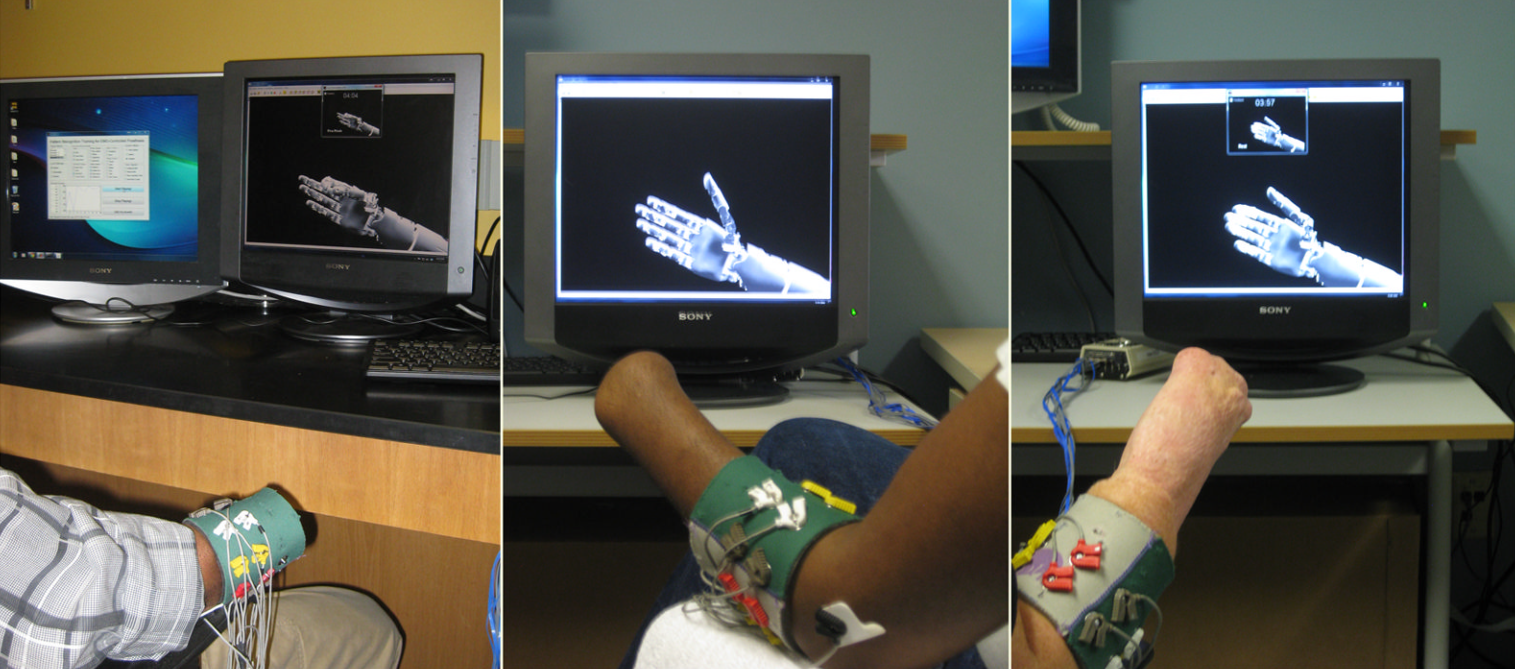
\includegraphics[width=.8\textwidth]{figures/xBackground/PowellUserTraining}  
	\caption{Illustration of the experimental setup used in \cite{Powell2014}. Initially the user tries to mimic the movement, shown by a prosthesis in the interface, with their phantom limb, thus activating muscles in their residual limb corresponding to the instructed movement. The EMG produced is recorded and used to train a control system. The control system then enables the user to control the prosthesis in the interface, and receive feedback on which movement is performed.}
	\label{fig:PowellUserTraining} 
\end{figure}

Pan et al. \cite{Pan2017} provided a visual feedback of an arrow to be moved on a 2D plane. The arrow was controlled by two DOF's; one controlled the horizontal position of the arrow, while the other could rotate the arrow \cite{Pan2017}. Fang et al. \cite{Fang2017} provided real-time visual feedback of subjects performed movement in relation to the classes defined in the system. The feedback visualized a map of clusters of different classes which subjects could match the position of a cursor to. When subjects could match the cursor to the centroid of a cluster the performed movement corresponded the best with the class of that movement. \cite{Fang2017} An illustration of the experimental setup used in \cite{Fang2017} can be seen in \figref{fig:FangUserTraining}. All studies observed an improvement in user performance after being exposed to focused user training with visual feedback.

\begin{figure}[H]                 
	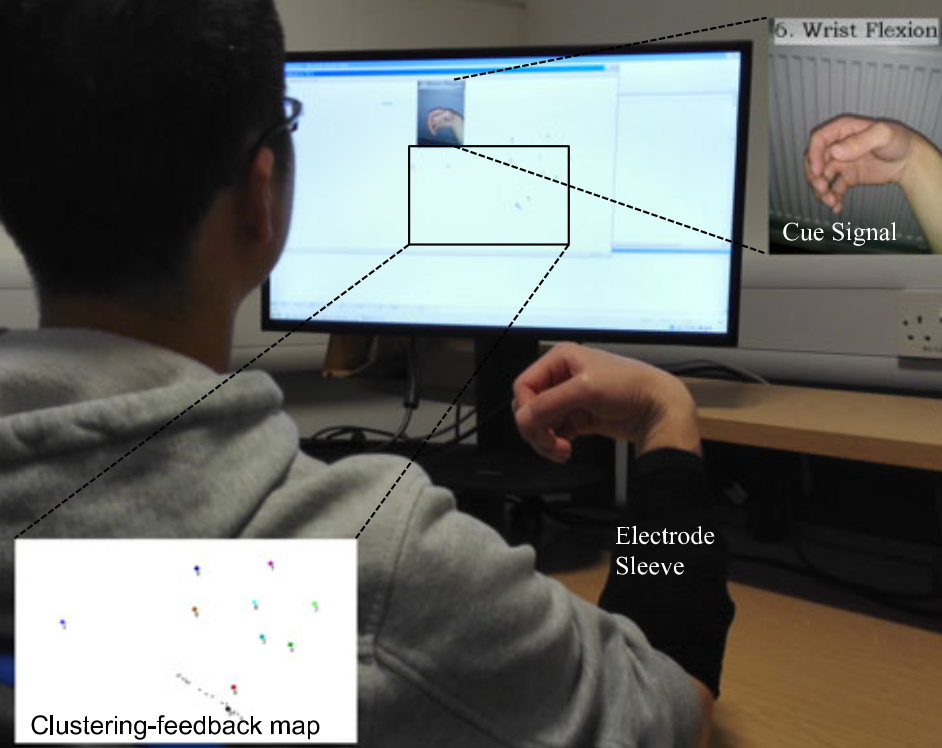
\includegraphics[width=.7\textwidth]{figures/xBackground/FangUserTraining}  
	\caption{An illustration of the experimental setup used in \cite{Fang2017}. The user received a cue on which movement should be performed. The user then had to fit a cursor, controlled by the user, to the centroid of the cluster points corresponding to the instructed movement in a clustering-feedback map.}
	\label{fig:FangUserTraining} 
\end{figure}



%A 2013 study by Scheme et al. \cite{Scheme2013} proposed a novel approach of utilizing confidence-based rejection to improve system training of myoelectric control. Here a classification control scheme was provided with confidence scores to assist in acceptance or rejection of the class output. The confidence scores were calculated from a modification of Bayes' theorem. Scheme et al. \cite{Scheme2013} showed a significant improvement in performance with the use of the rejection-capable system when compared to the normal classification scheme. A similar approach could be used in user training by providing the confidence scores of the classification to the user as a form of visual feedback. 
